\section{Cloud-native Architecture}

\begin{frame}{Cloud-Native Architecture}
    \begin{itemize}
        \item Bisher: Vorab-Allokation von Ressourcen
        \item Jetzt: Allokation genau dann, wenn notwendig
        \item Cloud-Native: Explizit für die Cloud entwickelte Applikationen \cite{cloudNative}
        \item Annahme: Infrastruktur ist in ständigem Wandel
        \item Folgerung: Infrastruktur auslagern - an Cloud-Vendor
        \begin{itemize}
            \item Globale Nutzung durch Geo-Redundanz: Starke Verteilung und hohe Verfügbarkeit
            \item Auto-Scaling: Dynamische Skalierung basierend auf Nachfrage
            \item Pay-as-you-go, Scale-to-zero: Nur verwendete Ressource wird bezahlt
            \item Zero Downtime
        \end{itemize}
    \end{itemize}
\end{frame}

\begin{frame}{Cloud-Native Architecture: Technologie}
    \begin{itemize}
        \item Containerisierung: Jede Komponente eines Systems ist Container
        \item Dynamische Orchestrierung: Aktives Container-Management zur Ressourcenoptimierung
        \item Microservice-Architektur ist Fundament - ergänzt durch Cloud-Dienste
        \item Fully Managed Cloud-Services: Business-Logik statt Infrastruktur
    \end{itemize}
\end{frame}

\begin{frame}{Cloud-Native Architecture: Beispiel E-Commerce}
    \begin{figure}[!h]
        \centering
        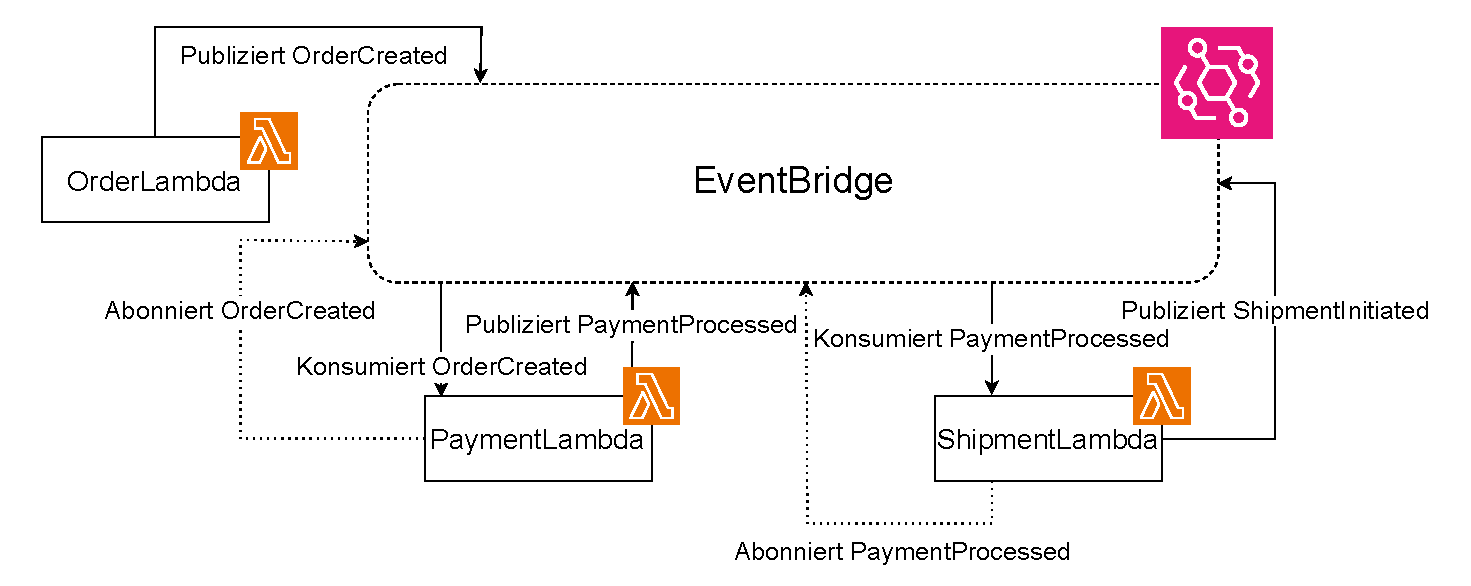
\includegraphics[scale=0.5]{imglib/cloud-native/cloud-native-ecommerce.drawio}
        \caption{E-Commerce-Beispiel mit Cloud-Native Architecture in AWS}
        \label{fig:cloudnativeecommerce}
    \end{figure}
\end{frame}

\begin{frame}{Cloud-Native Architecture: Agilität}
    \begin{itemize}
        \item Alle agilen Vorteile von Microservice- und Event-Driven Architecture
        \item Fokus auf Business-Logik \& einfaches Deployment $\Rightarrow$ Kurze Iterationen
        \item Maximale Flexibilität für Nachfrage durch Auto-Scaling
        \item Finanzielle Agilität: Pay-as-you-go
        \item Aber: Kostenrisiken durch Auto-Scaling und Pay-as-you-go
        \item Achtung: Vendor-Lock-In durch proprietäre Fully Managed Cloud-Services
    \end{itemize}
\end{frame}
